\documentclass[11pt]{article}
\usepackage[letterpaper,landscape,margin=0.6in]{geometry}
\usepackage{booktabs,graphicx}
\setlength{\parindent}{0pt}
\setlength{\parskip}{5pt}
\begin{document}
\begin{center}\Large\textbf{Revealed-preference distance by rationality role and group outcomes}\end{center}
\small
Compare each member's normalized distance to the group, $\widehat I_{ig}$, using the same index as the paper.
Lower distance means greater relative alignment with group choices. Roles use individual CCEI separately in each wave.
\begin{center}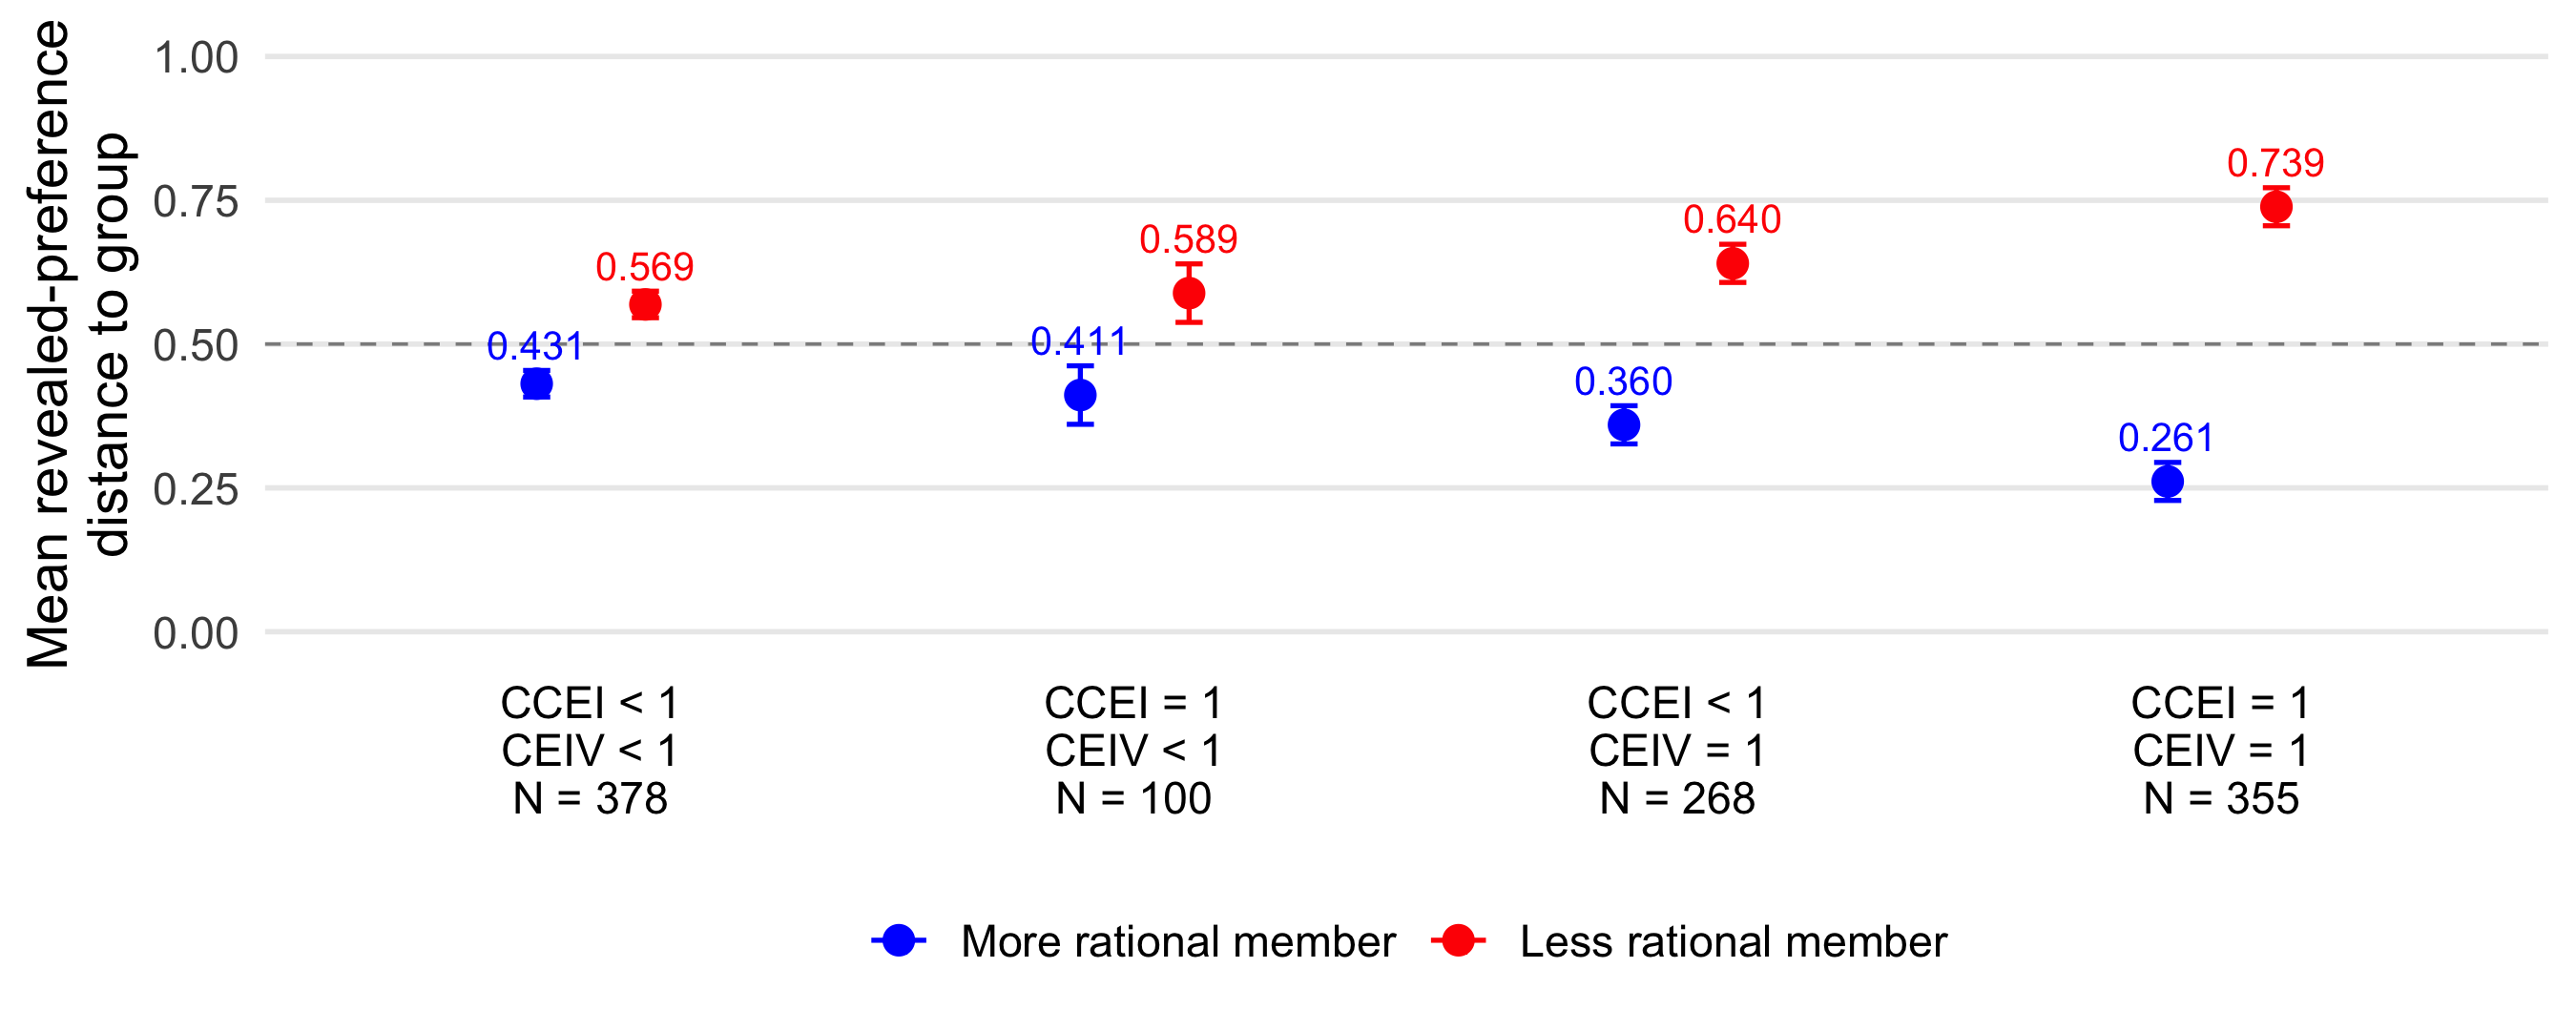
\includegraphics[width=0.81\textwidth]{distance_by_role.png}\end{center}
\begin{center}\small\begin{tabular}{lrrrrrr}\toprule
Group outcomes & More rational & Less rational & Less minus more & Pair-waves & CCEI ties excluded & Missing excluded\\\midrule
CCEI$<1$, CEIV$<1$ & 0.431 & 0.569 & 0.138 & 378 & 37 & 0\\
CCEI$=1$, CEIV$<1$ & 0.411 & 0.589 & 0.177 & 100 & 17 & 0\\
CCEI$<1$, CEIV$=1$ & 0.360 & 0.640 & 0.281 & 268 & 31 & 1\\
CCEI$=1$, CEIV$=1$ & 0.261 & 0.739 & 0.478 & 355 & 114 & 3\\
\bottomrule\end{tabular}\end{center}
\textbf{Reading the pattern.} The more rational member is closer to group choices in all four categories (paired
within-category differences: $p<0.001$ throughout). The difference is largest when both group indices equal one.
Within CEIV$=1$, the more rational member's mean distance is 0.261 when CCEI$=1$, compared with 0.360 when CCEI$<1$;
the difference is $-0.098$ ($p<0.001$). The less rational member's distance increases by the same amount.

\footnotesize
\textit{Notes:} Unadjusted descriptive means, pooling both waves without an RA-gap restriction. Bars are 95\% confidence
intervals clustered by 64 classes, accounting for both members and repeated waves. Among 1,304 eligible pair-waves,
199 have individual CCEIs tied within $10^{-9}$; four additional untied pair-waves lack both distances. The plotted sample
contains 1,101 pair-waves (2,202 member-waves). ``Missing excluded'' refers only to untied pairs; ties are counted separately.
Categories match Figure 6; CCEI/CEIV values at least $1-10^{-9}$ count as one.

The two distances sum to one within each pair-wave, so the two role means are complementary and reflect one comparison.
The index measures relative member-to-group closeness, not absolute disagreement between the two individuals and not
aggregation weights. A higher normalized distance for the less rational member does not establish greater absolute
distance from the group. Outcome categories and distances are constructed from related choice data; the associations
do not identify a decision process. Comparisons are exploratory, with no multiple-testing adjustment.
\end{document}
